\input{chapter-header.tex}

% ===========================================================================
\chapter{VirtuaTalk: An Infrastructure for Runtime Evolution}
\minitoc
% ===========================================================================
\introduction
% ===========================================================================

% ===========================================================================
\section{A Virtual Runtime System in a Nutshell}

We propose the introduction of first class object runtime systems, namely \emph{object spaces}, to aid and support the evolution of object-oriented software.
Object spaces encapsulate an object runtime system and provide a high-level API to query and modify it. An object space consists, then, on two main components: the object runtime system it represents, and the first class objects used for its manipulation. Figure \ref{fig:objectSpaceOverview} gives an overview of the relation between object runtime systems when using object spaces.

\begin{figure}[htb]
\begin{center}
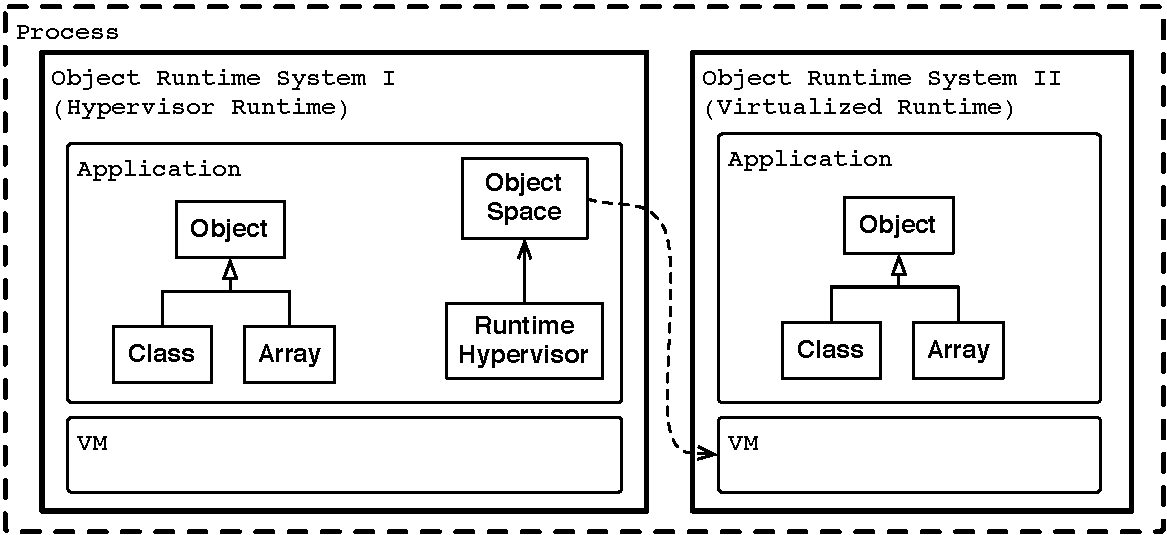
\includegraphics[width=.9\linewidth]{object_space_overview3}
\caption{Object from object runtime system I can manipulate through the Object Space library the object runtime system II.\label{fig:objectSpaceOverview}}
\end{center}
\end{figure}

The first advantage of using object spaces relies on the addition of a new level of abstraction, decoupling our client applications from the internal representation of the second runtime system. The runtime system under manipulation can reside \eg on the same operating system process, on a different process, or even on a simulated runtime system.

Second, it presents a uniform high-level API for the manipulation of its runtime system. This API provides services for the manipulation of execution, code and objects inside the object space~(cf. Sections \ref{sec:membrane} and \ref{sec:execution}). Through this API, an object space enforces safe communication between runtime systems~(cf. Section \ref{sec:communication}) and isolation~(cf. Section \ref{sec:isolation}).

%\begin{figure}[ht]
%\center
%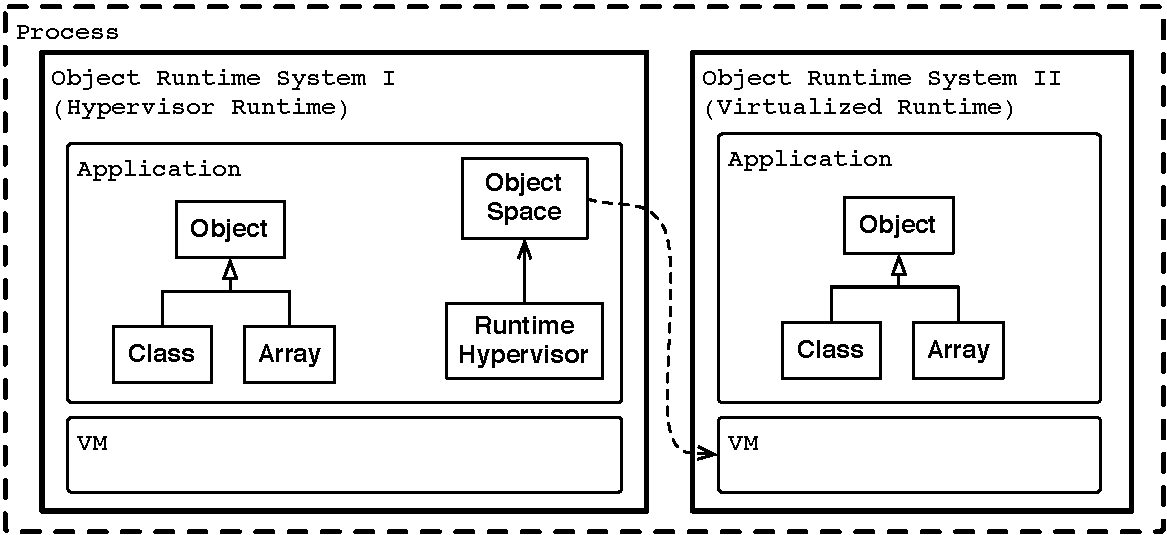
\includegraphics[width=.9\linewidth]{object_space_overview3}
%\caption{\textbf{Solution overview.} \label{fig:objectSpaceOverview}}
%\end{figure}

%A virtual Smalltalk image is an image living inside another Smalltalk image. The container image, the host, observes the virtual image and has complete control over it.
%The main idea is that such tasks difficult to perform due to the reflective architecture are handled by the host image. We transform the critical "self-brain surgery" tasks into safe "brain surgery" ones, by delegating them to another Smalltalk image.

%Oz is a virtual image model and implementation based on \objectspaces~\cite{Casa09a}. Casaccio et al. sketched \objectspaces to solve self-brain surgery. When doing self-brain surgery, the image under modification becomes a \emph{patient} of a \emph{surgeon} image. The patient is included inside the surgeon as an \objectspace. Through this \objectspace, the image gets manipulated by the surgeon, fixed and finally awoken.

%In figure \ref{fig:objectSpaceOverview} we can see an \objectspace represented as the graph within the dotted line, containing a guest smalltalk image a fa\c{c}ade object and a .

%An \objectspace appears as a first-class object which reifies a full Smalltalk image.
%An \objectspace is a fa\c{c}ade object the surgeon uses to reason about and act upon the patient Smalltalk image.

%In this paper, we extend \objectspaces to \textbf{virtual Smalltalk images}. We understand an \objectspace a a full Smalltalk image completely controllable from the outside. Then, an \objectspace exposes its object graph as well as other resources such as its complete execution or files.

%In this section we describe the concepts and design principles guiding our \objectspace solution for virtual Smalltalk images.
%\gp{come back here and finish this part!!!}

%\subsection{Object Spaces Overview} \label{sec:definitions}

%In Oz, an \objectspace is a subsystem of another image. It is an object graph composed by two main elements: a full Smalltalk image (cf. Section \ref{sec:isolation}) and a \emph{"membrane"} of objects controlling that image (cf. Section \ref{sec:membrane}). The image containing an \objectspace is its \emph{host}, while the \objectspace is its \emph{guest}.


%\begin{description}
%\item[Accessing well known objects.] Well known objects such as \ct{nil}, \ct{true} and \ct{false} can be get and set from an object space. The bootstrap process uses it during the well known instances initialization step. Once an object space is configured with such objects, it can execute code using them and overcome the \textbf{unicity hypothesis}.
%\begin{code}
%mirror getNil();
%mirror getTrue();
%mirror getFalse();
%
%void setNil(mirror aNilObject);
%void setTrue(mirror aTrueObject);
%void setFalse(mirror aFalseObject);
%\end{code}
%
%\item[Object allocation.] Object allocation operations provide support for the initialization of the guest language kernel. In particular, \ct{allocateObjectOfSize()} is the unsafe operation used to instantiate the first objects when there are no classes available.
%\begin{code}
%mirror allocateObjectOfSize(int size);
%mirror allocateObjectOfClass(mirror aClass);
%mirror compile(String sourceCode, mirror aClass);
%\end{code}

\section{Object Spaces: First-class Runtime Images} \label{sec:membrane}

An object space exposes its API through mirrors~\cite{Brac04b}. 


\subsection{Runtime Mirror}

\begin{description}
\item[Runtime system manipulation.] To initialize the classes in the guest language kernel, Oz provides with operations to install classes and obtain the list of classes installed.
\begin{code}
void installClass(mirror aClass);
List<mirror> getClasses();
\end{code}

\end{description}

\subsection{Low Level Mirrors}

Our object space solution involves two different kind of mirrorsMirrors mediate the interaction between guest and host language kernels to keep them \textbf{isolated} from each other \ie object references from the guest language kernel do not leak into the host language kernel and vice-versa. To ensure isolation, mirrors provide the following API to interact with the objects they wrap:

\begin{description}

\item[Class access.] Method installation and object manipulation is achieved by class access operations. In particular, the \ct{setClass()} operation is used in the first steps of the bootstrap process to close the main circularities and set the class of the \ct{nil} object.
\begin{code}
mirror getClass().
void setClass(mirror aClass).
\end{code}

\item[Internal state access.] Every object initialization of the bootstrap process is achieved by altering their internal state. Mirrors provide a low level API to get and set the fields of an object.
\begin{code}
mirror getInstanceVariable(String variableName).
void setInstanceVariable(String variableName, mirror anObject).
\end{code}


%\item[Code execution.] Oz provides with operations to manipulate the processes/threads of the guest language kernel. In particular, the \ct{runForTime()} operation will execute the guest language kernel with whichever processes it has installed, directly on the VM.
%\begin{code}
%List<mirror> getProcesses();
%mirror createProcessDoing(String expression);
%void runForTime(int milliseconds);
%\end{code}
%\caption{\textbf{Code of the Builder implementing the same logic as in \ct{Dictionary>>initialize}.}\label{code:logic_dup2}}
%\end{figure}
\end{description}

\subsection{High Level Mirrors}


% ===========================================================================

\section{Code Execution in not-yet Causally-Connected languages} \label{sec:execution}

An \objectspace's execution is fully controllable from the host. The host can introspect and modify an \objectspace processes via mirrors to obtain information such as the method currently on execution, the values on the stack or the current program counter. Besides from those reflective operations, an \objectspace provides also operations to suspend, resume or terminate existing processes, and to install new ones.

The \objectspace provides fine-grained control on the guest execution. An \objectspace controls the amount of CPU used by the guest image. \sd{can you do that for real? CPU control?}\gp{We can give an objectspace a window of 20ms to run and then we get back control so It's our decision if we give it 20 more or not :)}This way, a virtual image can be customized for scenarios like for example testing, CPU usage analysis, or old hardware simulation. For example, it may restrict its processes to run during only 300 milliseconds every second for either.

\gp{example!}

\begin{description}
\item[Code execution.] Oz provides with operations to manipulate the processes/threads of the guest language kernel. In particular, the \ct{runForTime()} operation will execute the guest language kernel with whichever processes it has installed, directly on the VM.
\begin{code}
List<mirror> getProcesses();
mirror createProcessDoing(String expression);
void runForTime(int milliseconds);
\end{code}
%\caption{\textbf{Code of the Builder implementing the same logic as in \ct{Dictionary>>initialize}.}\label{code:logic_dup2}}
%\end{figure}
\end{description}

\section{Communication and Isolation} \label{sec:communication}\label{sec:isolation}

\gp{rewrite: cross message sends, literal translation, and boundary checks}

As explained in Section \ref{sec:isolation}, an objectspace is an isolated object graph in the sense that from the guest image there is no way to reach host objects. However, the opposite relation is possible: the host can manipulate completely the \objectspace.

The communication mechanism between host and guest images is based on the \emph{injection of objects} into the \objectspace. The host may install from simple literal objects such as strings or numbers, up to more complex objects like classes, methods. An \objectspace permits to \emph{send messages to objects} inside itself by injecting process with the specified code. Injected processes may have any arbitrary expression. The membrane objects can retrieve the result from the process' context once the execution is finished.

The \objectspace membrane ensures that object injection honors the transitive closure property. On one side, literal objects from the host are automatically translated to their representation in the \objectspace. An \objectspace implements the operations to transform literal objects (numbers, strings, symbols, some arrays and byte arrays) \emph{from and to} its internal representation.

On the other side, non literal objects are actually not created in the host and injected in the \objectspace. Non literal objects are directly created in the \objectspace, so the task of injecting the new object inside a graph is safe.

\gp{example!}



Note from the signatures presented that all mirror operations will return a mirror in exchange, and so, interaction with other objects inside the object space is mediated by Oz. Mirrors could give and revoke permissions on the wrapped object and enforce invariants to keep the model consistent~\cite{Teru13a}.
Oz provides also specific kinds of mirrors with high level APIs to manipulate objects with a specific format and/or behavior such as classes, methods, activation records or processes. We do not cover high level mirrors in this paper because they are not relevant to the bootstrap process.

\gp{next is old, see how to merge}

The manipulation of objects inside the \objectspace image cannot be achieved with a traditional message send mechanism. In the normal case, when a message send is performed, the virtual machine takes the selector symbol of the message and lookups in the class hierarchy method dictionaries of the receiver until it finds a method with the \emph{same}~(identical) selector. In our scenario, both host and guest images contain their own \ct{Symbol} class and symbol table. Then, when performing a \emph{cross image-message send} the method lookup mechanism takes a selector symbol from the host, lookups into the guest receiver's hierarchy, and finally fails because  the selector in the guest is (while maybe equals) not identical to the selector in the host. Also, forcing a \emph{cross image-message send} by using a guest's selector can leak host references to the guest: activating a guest method from the host gives the guest complete access to the host through the \ct{thisContext} special variable which reifies the stack on-demand.

To encapsulate and control the basic object manipulation, the object space fa\c{c}ade object provides mirrors~\cite{Brac04b}. Mirrors hide the internal representation of the objects inside the objectspace and expose reflective behavior. The guest is not aware of the existence of these mirrors.

All objects inside an \objectspace and reachable by reference can be retrieved by host's objects through the \objectspace facade and mirrors. 
There is no limitation nor restriction for object access. 
The host manipulates all objects in a homogeneous way through their mirrors. 

Additionally, specific mirrors are provided to manipulate objects with a specific format and/or behavior such as \ct{Class}, \ct{Metaclass}, \ct{MethodDictionary}, \ct{CompiledMethod}, \ct{MethodContext}, and \ct{Process}.

\section{Explicit Runtime State}

% =============================================================================
\input{chapter-footer.tex}